\documentclass[11pt]{article}
\usepackage{amsmath}
\usepackage{amssymb}
\usepackage{algpseudocode,algorithm}
\usepackage{graphicx}
\usepackage{psfrag,color}
\usepackage{fullpage}
\usepackage{epsfig}
\usepackage{graphicx}
\usepackage{verbatim}
\usepackage{listings}

\setlength{\topmargin}{-0.7in}
\setlength{\textwidth}{6.5in}
\setlength{\oddsidemargin}{0.0in}
\setlength{\textheight}{10.0in}
\setlength{\parindent}{0in}

\renewcommand{\baselinestretch}{1.2}
\renewcommand\arraystretch{1.5}
\newcommand{\problem}[1]{ \medskip \pp $\underline{\rm Problem\ #1}$\\ }


\pagestyle{empty}

\def\pp{\par\noindent}


\begin{document}

\begin{flushright}
{\bf STAT GR5703---Spring 2020}
\end{flushright}
\begin{flushleft}
Group: Zining Fan, Mutian Wang, Siyuan Wang\\
UNI: zf2234, mw3386, sw3418\\
\end{flushleft}

\bigskip
\centerline{\bf Graded Homework 1 - Exercise 5}

\bigskip
\begin{enumerate}
%5.1
\item The author adopts a probabilistic approach, instead of a trandional social deterministic model, to explain the phenomenon that many independent techno-scientific discoveries/inventions occurred simultaneously in the history. \par
The main statistical model used by the author is Poisson distribution, an approximation to binomial distribution. Suppose there are $n$ people working on a techno-scientific problem, and each person has the probability $p$ to discover/invent something, then the number of repeats, $X$, is approximately a Poisson random variable. \par
Generally speaking, this model is reasonable. Intuitively, in this scenario, $n$ should be large and $p$ should be small, so Poisson distribution is a reasonable approximation. Also the CDF of Poisson distribution is much simpler than that of binomial distribution. More importantly, such approximation reduces the number of parameters from 2 to 1. However, the probability for each person to succeed is certainly not the same, and one person might have influence on others. In addition, the historical data of $X=0$ and 1 are missing/inadequate, as mentioned in the article. Despite all these problems, this model is fairly good.

%5.2
\item This is 1-truncated Poisson distribution, also known as conditional Poisson distribution. It is the Poisson distribution conditioned on the event $Y \ge 2$. The advantage is that 1-truncated Poisson distribution fits the data better, because it does not depend on $Y=0$ and 1 and the historical data do not have such information.

%5.3
\item
\begin{equation*}
\begin{split}
E[Y] &= \sum\limits_{k=2}^{\infty} \left( 
\frac{ke^{-\mu}\mu^k}{k!} \cdot \frac{1}{1-e^{-\mu}-\mu e^{-\mu}} \right) \\
&= \frac{1}{1-e^{-\mu}-\mu e^{-\mu}} \cdot \left(
 \sum\limits_{k=0}^{\infty} \frac{ke^{-\mu}\mu^k}{k!} - 0\cdot e^{-\mu}-\mu e^{-\mu} \right) \\
&= \frac{\mu-\mu e^{-\mu}}{1-e^{-\mu}-\mu e^{-\mu}}
\end{split}
\end{equation*}

\begin{equation*}
\begin{split}
E[Y^2] &= \sum\limits_{k=2}^{\infty} \left( 
\frac{k^2e^{-\mu}\mu^k}{k!} \cdot \frac{1}{1-e^{-\mu}-\mu e^{-\mu}} \right) \\
&= \frac{1}{1-e^{-\mu}-\mu e^{-\mu}} \cdot \left(
 \sum\limits_{k=0}^{\infty} \frac{k^2e^{-\mu}\mu^k}{k!} - 0\cdot e^{-\mu}-\mu e^{-\mu} \right) \\
&= \frac{\mu+\mu^2-\mu e^{-\mu}}{1-e^{-\mu}-\mu e^{-\mu}}
\end{split}
\end{equation*}

\begin{equation*}
\begin{split}
var(Y) &= E[Y^2] - E[Y]^2 \\
&= \frac{\mu+\mu^2-\mu e^{-\mu}}{1-e^{-\mu}-\mu e^{-\mu}} - \left(
\frac{\mu-\mu e^{-\mu}}{1-e^{-\mu}-\mu e^{-\mu}} \right)^2 \\
&= \frac{\mu-2\mu e^{-\mu}+\mu e^{-2\mu}-\mu^3e^{-\mu}}{(1-e^{-\mu}-\mu e^{-\mu})^2}
\end{split}
\end{equation*}

%5.4
\item 
\begin{equation*}
\begin{split}
\because L(\mu; Y) &= \prod\limits_{i=1}^n \frac{e^{-\mu}\mu^{Y_i}}{Y_i!} \cdot \frac{1}{1-e^{-\mu}-\mu e^{-\mu}} \\
&= \left(\frac{e^{-\mu}}{1-e^{-\mu}-\mu e^{-\mu}}\right)^n \cdot \frac{\mu^{\sum Y_i}}
{\prod Y_i!} \\
&= \left(\frac{1}{e^{\mu}-1-\mu}\right)^n \cdot \frac{\mu^{\sum Y_i}}
{\prod Y_i!} \\
\therefore \ln L(\mu; Y) &= -n \cdot \ln (e^\mu - 1 - \mu) 
- \sum\limits_{i=1}^n \ln Y_i! + \ln \mu \cdot \sum\limits_{i=1}^n Y_i
\end{split}
\end{equation*}

\begin{center}
  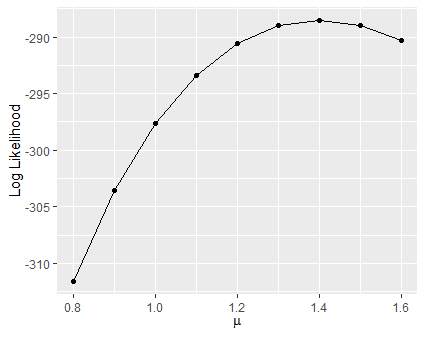
\includegraphics[width=0.7\linewidth]{Q5.png}
\end{center}

%5.5
\item
The chosen algorithm is a built-in function in R, $nlm()$. It is the non-linear minimization using a Newton-type algorithm. We use this function to minimize the negative log likelihood.

\begin{lstlisting}[frame=single]
data <- c(rep(2,179), rep(3,51), rep(4,17), rep(5,6), 
         rep(6,8), rep(7,1), rep(9,2))
n <- length(data)
fun <- function(mu){
 n*log(exp(mu)-1-mu) + sum(log(factorial(data))) - log(mu)*sum(data) 
}
nlm(fun, mu <- 1, hessian = T)
\end{lstlisting}

\verbatiminput{Q5.txt}

%5.6
\item Since MLE is always asymptotically normally distributed, we have 
$$\sqrt{n}\left( \hat{\mu}_{\mathsf{MLE}} -\mu \right)  \xrightarrow[n\rightarrow \infty]{D} 
N\left( 0,I(\mu)^{-1} \right)$$

\begin{equation*}
\begin{split}
I(\mu) &= -E[\frac{\partial^2}{(\partial \mu)^2} \ln L(\mu;Y_1)] \\
&=\frac{e^\mu-\mu e^\mu - 1}{(e^\mu-\mu-1)^2} + \frac{E[Y_1]}{\mu^2} \\
&=\frac{e^\mu-\mu e^\mu - 1}{(e^\mu-\mu-1)^2} + 
\frac{\mu-\mu e^{-\mu}}{1-e^{-\mu}-\mu e^{-\mu}} \cdot \frac{1}{\mu^2} \\
&= \frac{-\mu^2e^\mu + e^{2\mu} - 2e^\mu + 1}{\mu(e^\mu-\mu-1)^2}
\end{split}
\end{equation*}

$$\therefore \hat{\mu}_{ML} \xrightarrow[n\rightarrow\infty]{D} N\left( \mu, \frac{1}{nI(\mu)} \right)
\mbox{ where } I(\mu) = \frac{-\mu^2e^\mu + e^{2\mu} - 2e^\mu + 1}{\mu(e^\mu-\mu-1)^2}$$

%5.7
\item
Since we know the asymptotic distribution of $\hat{\mu}_{ML}$, we can construct a 0.95 asymptotic confidence interval as follows,
$$\left[\hat{\mu}_{ML}-\sqrt{\widehat{var}(\hat{\mu}_{ML})} \cdot z_{0.975},
\hat{\mu}_{ML}+\sqrt{\widehat{var}(\hat{\mu}_{ML})} \cdot z_{0.975}   \right]$$
If we plug in values obtained earlier ($n=264, \hat{\mu}_{ML}=1.398$), we can get the confidence interval, 
$$[1.197427, 1.598573]$$

%5.8
\item Generally speaking, this is a reasonable way to estimate $\mu$. Since the author picked the value of $\mu$ with the minimal $\chi^2$ value, the chosen $\mu$ should best fit the data. \par
Yet we also have some doubts. Manually tuning the value of $n_\mu$ for each value of $\mu$ sounds strange to us. The optimum $\mu$ might be influenced by the author and cannot reflect the truth. Anyway, the result of this technique turns out quite good. \par
Because of the human intervention, we cannot calculate this estimator's bias, consistency or variance.

%5.9
\item The results are almost identical. Simonton's estimate of $\mu$ is 1.4, while $\hat{\mu}_{\mathsf{MLE}}=1.398391$. \par
However, we can have more information about the maximum likelihood estimator, such as its distribution, bias, variance, consistency, etc. \par
Also, we only need to find a value of $\mu$ that maximizes the log likelihood, whereas we have to find the best pair $(\mu, n_{\mu})$ that minimizes the $\chi^2$ value. So it seems the MLE method is somewhat less complex.



\end{enumerate}
\end{document}